\subsection*{Floodfill}

\subsubsection*{Motode}
Floodfill omhandler detektion af områder i et billet som har samme farve
eller en farve som ligger inde få en vis afvigelse af den originale
farve. Der vælges en pixel i billet, denne pixel har farven (r,g,b). Ud
fra denne pixel, detekter de pixels som er nabolaget til pixlen, i
lodret og vandret bane. Som se på billedet $\label{floodfill1}$.

\begin{figure}[h]
	\begin{center}
		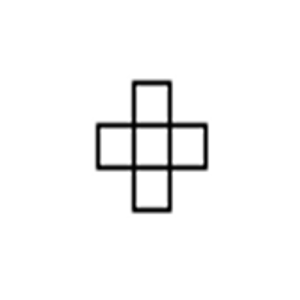
\includegraphics[scale=0.42,angle=0]{afsnit/vores_implementation/billeder/flood_fill/floodfill1}
	\end{center}
	\caption[]{Måden flodfill arbejder med pixelsene i billedet}
	\label{floodfill1}
\end{figure}

(1). Den mideste pixlen, start pixlen bliver sat sat med en flag,
betejnet med at pixlen bliver tegnet rød og bliver favet. nabopixlene få
flaget blå da de skal tjækkes på om faven er inde for gransen, hvis de
ikke har nogle flag i forvejen.

\begin{figure}[h]
	\begin{center}
		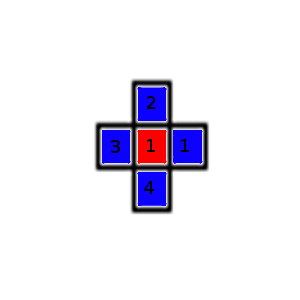
\includegraphics[scale=0.42,angle=0]{afsnit/vores_implementation/billeder/flood_fill/floodfill2}
	\end{center}
	\caption[]{Efter step 1}
	\label{floodfill2}
\end{figure}

(2). For vært blådt flag bliver der tjekket om faven er inde for
gransen, hvis den er det, kommer pixlen ind i et liste og et grøndt flag
bliver sat, betegnet som den grønde pixlen og nummeret.

\begin{figure}[h]
	\begin{center}
		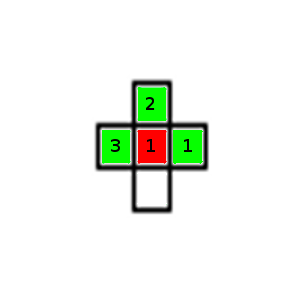
\includegraphics[scale=0.42,angle=0]{afsnit/vores_implementation/billeder/flood_fill/floodfill3}
	\end{center}
	\caption[]{Efter step 2}
	\label{floodfill3}
\end{figure}

(3). En af de grønde flag bliver sat til den nye startpixel og metode
(1) til (3) bliver gentaget ind til der ikke er flere grønde flag 

\begin{figure}[h]
	\begin{center}
		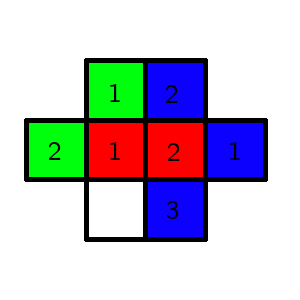
\includegraphics[scale=0.42,angle=0]{afsnit/vores_implementation/billeder/flood_fill/floodfill4}
	\end{center}
	\caption[]{Efter step 1 af en ny gemmen kørsel af floodfill}
	\label{floodfill4}
\end{figure}

På denne måde iterere metoden sig i gemmen alle de pixels som ligger
inde for en vist nivo af start farven. Denne metode kan gøres på to
måde, enden kan man regne nivoet som faven må variere med ud fra farven
som start pixlen har, eller fra den nye pixel som bliver fundet i step
(3).

\subsubsection*{Overvejelser}
Som beskravet i slutningen af metode, forekommere der 2 måder. ved at
regne varianten ud fra start pixlen, få metode til at indskranke sig en
del, og ikke komme inde i alle hjørner af en ragion, tilgængeld har
metode svære ved at tegne over kanter og komme ind i en anden ragioner.
Ved at arbejde med metoden som regner på den nye pixels farve, få man en
metode som få meget af ragionen med, og som kan overskue at en ragion
kan skifte farve langsomt i forhold til solens position eller små skift
i ragionen. tilgængel er denne fremgangs måde ret følsom, og kommer
nemmer til at flyde over ragionen.

\subsubsection*{Ydre overvejelser}
For at få denne metode til at virke på 25000 billeder, hvor en del af
billederne ikke har samme farve tone eller er blevet falmet. Må der
udregnes, for vært billedet, hvad for en varians i fave der skal bruges.
